% Exact face-to-node correspondence for the input panel of Figure 3.
% The unchanged raster underneath supplies the two GNN branches and fusion path.
\begingroup
\newdimen\figthreeunit
\figthreeunit=\dimexpr\linewidth/1250\relax
\begin{tikzpicture}[x=\figthreeunit,y=\figthreeunit]
  \node[anchor=south west,inner sep=0,outer sep=0] at (0,0)
    {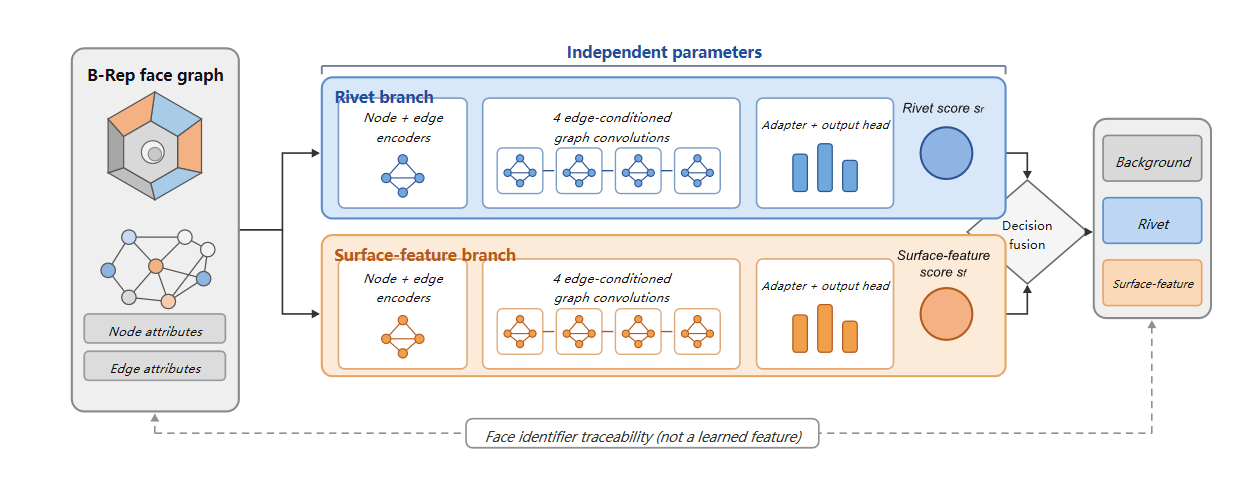
\includegraphics[width=\linewidth]{figures/fig_class_specific_gnn_architecture_v3.png}};

  % Replace only the input panel. A shared B-Rep edge becomes one graph edge.
  \begin{scope}[yshift=34\figthreeunit]
  \path[fill=white] (69,45) rectangle (241,415);
  \draw[rounded corners=13,fill=gray!9,draw=gray!55,line width=1.5\figthreeunit]
    (71,48) rectangle (239,412);
  \node[font=\sffamily\bfseries\fontsize{6.6}{7.5}\selectfont] at (155,389)
    {B-Rep face graph};

  % Four faces of a local B-Rep surface patch, viewed obliquely.
  \path[fill=blue!22,draw=gray!65,line width=1.1\figthreeunit]
    (101,351)--(153,366)--(151,322)--(101,308)--cycle;
  \path[fill=orange!38,draw=gray!65,line width=1.1\figthreeunit]
    (153,366)--(209,349)--(209,305)--(151,322)--cycle;
  \path[fill=gray!35,draw=gray!65,line width=1.1\figthreeunit]
    (101,308)--(151,322)--(151,280)--(101,265)--cycle;
  \path[fill=blue!46,draw=gray!65,line width=1.1\figthreeunit]
    (151,322)--(209,305)--(209,264)--(151,280)--cycle;
  \draw[draw=blue!75!black,line width=2.5\figthreeunit]
    (153,366)--(151,322);
  \node[font=\sffamily\bfseries\fontsize{6.3}{7}\selectfont] at (127,338) {F1};
  \node[font=\sffamily\bfseries\fontsize{6.3}{7}\selectfont] at (181,337) {F2};
  \node[font=\sffamily\bfseries\fontsize{6.3}{7}\selectfont] at (127,294) {F3};
  \node[font=\sffamily\bfseries\fontsize{6.3}{7}\selectfont] at (181,292) {F4};

  \node[font=\sffamily\fontsize{5.3}{6}\selectfont,text=black!70]
    at (155,245) {Shared edge $\rightarrow$ link};

  % F1--F4 and F2--F3 meet only at a vertex, so no diagonal graph edge exists.
  \draw[draw=gray!70,line width=1.2\figthreeunit] (121,214)--(121,166);
  \draw[draw=gray!70,line width=1.2\figthreeunit] (188,214)--(188,166);
  \draw[draw=gray!70,line width=1.2\figthreeunit] (121,166)--(188,166);
  \draw[draw=blue!75!black,line width=2.5\figthreeunit] (121,214)--(188,214);
  \foreach \x/\y/\name/\colour in {
    121/214/F1/blue!22,
    188/214/F2/orange!38,
    121/166/F3/gray!35,
    188/166/F4/blue!46
  } {
    \node[circle,minimum size=27\figthreeunit,inner sep=0,
      draw=gray!70,fill=\colour,line width=1.2\figthreeunit,
      font=\sffamily\bfseries\fontsize{5.8}{6.5}\selectfont]
      at (\x,\y) {\name};
  }

  \draw[rounded corners=4,fill=gray!16,draw=gray!55,line width=1.1\figthreeunit]
    (84,116) rectangle (226,145);
  \node[font=\sffamily\itshape\fontsize{5.6}{6.5}\selectfont]
    at (155,130) {Node attributes};
  \draw[rounded corners=4,fill=gray!16,draw=gray!55,line width=1.1\figthreeunit]
    (84,80) rectangle (226,109);
  \node[font=\sffamily\itshape\fontsize{5.6}{6.5}\selectfont]
    at (155,94) {Edge attributes};
  \end{scope}
\end{tikzpicture}
\endgroup
